% Author: Savin Ivan xsavini00
% Author: Turar Nurdaulet xturarn00
% Author: Krasovskyi Oleh xkrasoo00 
% Author: Popov Albert xpopov10 


\documentclass[a4paper, 11pt]{article}


\usepackage[czech]{babel}
\usepackage[utf8]{inputenc}
\usepackage[left=2cm, top=3cm, text={17cm, 24cm}]{geometry}
\usepackage[unicode,pdftitle={Překladač jazyka IFJ24},hidelinks]{hyperref}
\usepackage{times}
\usepackage{verbatim}
\usepackage{enumitem}
\usepackage{graphicx} % vkládání obrázků
\usepackage{longtable}
\usepackage{amsmath}
\hypersetup{
	colorlinks = true,
	hypertexnames = false,
	citecolor = red
}


\newcommand{\RNum}[1]{\uppercase\expandafter{\romannumeral #1\relax}} % makro na sázení římských čísel


\begin{document}


	%%%%%%%%%%%%%%%%%%%%%%%%%%%%%%%% Titulní stránka %%%%%%%%%%%%%%%%%%%%%%%%%%%%%%%%
	\begin{titlepage}
		\begin{center}
			
\includegraphics[width=0.77\linewidth]{FIT_logo.png} \\

			\vspace{\stretch{0.382}}

			\Huge{Projektová dokumentace} \\
			\LARGE{\textbf{Implementace překladače imperativního jazyka IFJ24}} \\
			\Large{Tým xpopov10, varianta vv-BVS}
			\vspace{\stretch{0.618}}
		\end{center}

		\begin{minipage}{0.4 \textwidth}
			{\Large \today}
		\end{minipage}
		\hfill
		\begin{minipage}[r]{0.6 \textwidth}
			\Large
			\begin{tabular}{l l l}
				\textbf{Popov Albert} & \textbf{(xpopov10)} & \quad 25\,\% \\
				Krasovskyi Oleh & (xkrasoo00) & \quad 25\,\% \\
				Savin Ivan & (xsavini00) & \quad 25\,\% \\
				Turar Nurdaulet & (xturarn00) & \quad 25\,\% \\
			\end{tabular}
		\end{minipage}
	\end{titlepage}



	%%%%%%%%%%%%%%%%%%%%%%%%%%%%%%%% Úvod %%%%%%%%%%%%%%%%%%%%%%%%%%%%%%%%
	\pagenumbering{arabic}
	\setcounter{page}{1}

	\section{Úvod}

	Cílem projektu bylo vytvořit program v jazyce C, který načte zdrojový kód zapsaný ve zdrojovém jazyce IFJ24,
    jenž je zjednodušenou podmnožinou imperativního programovacího jazyka Zig 0.13, a přeloží jej do cílového jazyka IFJcode24 (mezikód).
    
    Program funguje jako konzolová aplikace, která načítá zdrojový program ze standardního vstupu a generuje
    výsledný mezikód na standardní výstup nebo v případě chyby vrací odpovídající chybový kód.



    %%%%%%%%%%%%%%%%%%%%%%%%%%%%%%%% Práce v týmu %%%%%%%%%%%%%%%%%%%%%%%%%%%%%%%%
	\section{Práce v~týmu}

	\subsection{Způsob práce v~týmu}

	Na začátku projektu jsme úkol rozdělili do 4 hlavních bloků a jednali podle vzájemné interakce kódů. V případě, že se něčí práce zdála méně důležitá, tato osoba pomáhala ostatním nebo psal testy.
	\subsubsection{Verzovací systém}

	Pro správu souborů projektu jsme používali verzovací systém Git. Jako vzdálený repositář jsme používali \mbox{GitHub}.

	Git nám umožnil pracovat na více úkolech na projektu současně v~tzv. větvích. Většinu úkolů jsme nejdříve připravili
	do větve a~až po otestování a~schválení úprav ostatními členy týmu jsme tyto úpravy začlenili do hlavní
	vývojové větve.

	\subsubsection{Komunikace}

	Komunikace probíhala v obecné konverzaci nebo v soukromých zprávách.

	Ke konci projektu jsme se setkali, abychom ukázali, jak naše programové bloky fungují, s cílem najít chyby a zvýšit porozumění projektu ostatním účastníkům.


	\subsection{Rozdělení práce mezi členy týmu}

	Práci na projektu jsme si rozdělili rovnoměrně s~ohledem na její složitost a~časovou náročnost.
	Každý tedy dostal procentuální hodnocení 25\,\%.
	Tabulka shrnuje rozdělení práce v~týmu mezi jednotlivými členy.
	\bigskip
	\begin{table}[ht]
		\centering
		\begin{tabular}{| l | l |}
			\hline
			Člen týmu & Přidělená práce \\ \hline
			\textbf{Popov Albert} & \begin{tabular}{l} vedení týmu, testování, syntaktická analýza  \end{tabular} \\
			Vojtěch Hertl & \begin{tabular}{l} sémantická analýza, testování \end{tabular} \\
			Savin Ivan & \begin{tabular}{l}lexikální analýza  , dokumentace,  testování \end{tabular} \\
			Turar Nurdaulet & \begin{tabular}{l} generování cílového kódu, organizace práce, testovaní, struktura projektu\end{tabular} \\ \hline
		\end{tabular}
		\caption{Rozdělení práce v~týmu mezi jednotlivými členy}
		\label{table:rozdeleni_prace}
	\end{table}


	%%%%%%%%%%%%%%%%%%%%%%%%%%%%%%%% Návrh a implementace %%%%%%%%%%%%%%%%%%%%%%%%%%%%%%%%
	\section{Návrh a~implementace}

	Projekt jsme sestavili z~několika námi implementovaných dílčích částí, které jsou představeny v~této kapitole.
	Je zde také uvedeno, jakým způsobem spolu jednotlivé dílčí části spolupracují.

    \subsection{Struktura překladače}
    Překladač se skládá z následujících modulů:
    \begin{itemize}
        \item \textbf{Lexikální analyzátor (lexer):} Převádí zdrojový kód na tokeny
        \item \textbf{Parser:} Analyzuje tokeny pomocí syntaktických a sémantických pravidel a poté vytvoří abstraktní syntaktický strom (AST).
        \item \textbf{Generátor kódu:} Generuje z AST cílový kód.
    \end{itemize}
    
    Diagram konečného automatu pro lexer a LL tabulka budou přiloženy v~samostatných přílohách.

\section*{Folders structure}

\begin{itemize}
    \item \texttt{/docs}: Dokumentace projektu.
    \item \texttt{/include}: Hlavičkové soubory (\texttt{.h}) pro jednotlivé moduly.
    \item \texttt{/scripts}: Skripty pro spuštění a kontrolu projektu.
    \item \texttt{/src}: Implementace jednotlivých modulů překladače a hlavní soubor \texttt{main.c}.
    \item \texttt{/tests}: Testovací soubory a skripty na ověření funkčnosti.
\end{itemize}
    
	\subsection{Lexikální analýza}

    Jako první jsme začali s~lexikální analýzou. Zpočátku jsme počítali s~tím, že mezi všemi tokeny bude existovat nějaký oddělovací symbol, pomocí kterého lze zdrojový kód rozdělit na bloky. Každý blok by následně mohl být snadno přeložen na odpovídající tokeny. Později jsme však od této myšlenky museli upustit, protože v~některých případech bylo nutné implementovat příliš mnoho výjimek, což ztěžovalo rozšíření lexeru a zhoršovalo čitelnost kódu.  
    
    Nová verze lexikálního analyzátoru používá deterministický konečný automat (FSM). Hlavní funkce \texttt{run\_lexer()} načítá vstupní kód a spouští základní stav automatu. Nejprve se vyhledá první neprázdný znak a podle něj se přechází do příslušného stavu automatu. Po zpracování stavu se kód vrátí do funkce \texttt{run\_lexer()}, která pokračuje ve čtení, dokud není dosažen konec souboru.  
    
    Pro zpracování identifikátorů se nejprve přečtou povolené znaky. Po jejich přečtení se zkontroluje, zda se jedná o klíčové slovo nebo identifikátor. To umožňuje oddělit klíčová slova a vytvořit odpovídající znaky.
    
    Při zpracování čísel se čtou číslice, tečky a znak e/E. Pokud je posloupnost zadána správně, vytvoříme podle zadaných údajů token f64 nebo i32
    
    Celý lexikální analyzátor je implementován jako deterministický konečný automat podle předem vytvořeného diagramu, který bude přiložen v~příloze. Tento diagram specifikuje jednotlivé stavy a přechody mezi nimi, což usnadňuje údržbu a rozšíření lexeru v~případě potřeby.  

	\subsection{Syntaktická analýza}

	<< PUT YOUR TEXT HERE >>

	\subsubsection{Here is a subsection if needed}

	\texttt{OurCode.c}.

	Some text


	\subsection{Sémantická analýza}

	Sémantická analýza


	\subsection{Generování cílového kódu}

	Generování cílového kódu

	\subsubsection{Possible subsection}

    Some data


	


	%%%%%%%%%%%%%%%%%%%%%%%%%%%%%%%% Závěr %%%%%%%%%%%%%%%%%%%%%%%%%%%%%%%%
	\section{Závěr}

	Projekt nás zprvu trochu zaskočil svým rozsahem a~složitostí. Postupem času, až jsme získali dostatek
	znalostí o~tvorbě překladačů na přednáškách IFJ, jsme projekt začali řešit.

	Náš tým jsme měli sestaven velmi brzy, byli jsme již předem domluveni na komunikačních kanálech,
	osobních schůzkách a~na používání verzovacího systému, tudíž jsme s~týmovou prací neměli žádný
	problém a~pracovalo se nám společně velmi dobře.

	Na projektu jsme začali pracovat trochu později, takže jsme neměli časovou rezervu, ale nakonec
	jsme všechno stihli. Jednotlivé části projektu jsme řešili většinou individuálně za použití
	znalostí z~přednáškek nebo materiálů do předmětů IFJ a~IAL.

	V~průběhu vývoje jsme se potýkali s~menšími problémy týkajícími se nejasností v~zadání, ale
	tyto jsme vyřešili díky fóru k~projektu. Správnost řešení jsme si ověřili automatickými
	testy a~pokusným odevzdáním, díky čemuž jsme byli schopni projekt ještě více odladit.

	Tento projekt nám celkově přinesl spoustu znalostí ohledně fungování překladačů, prakticky nám
	objasnil probíranou látku v~předmětech IFJ a~IAL a~přinesl nám zkušennosti s~projekty tohoto rozsahu.

	%%%%%%%%%%%%%%%%%%%%%%%%%%%%%%%% Přílohy %%%%%%%%%%%%%%%%%%%%%%%%%%%%%%%%
	\clearpage
	\appendix


	%\section{Diagram konečného automatu specifikující lexikální analyzátor}
	%\begin{figure}[!ht]
	%	\centering
	%	\vspace{-1.2cm}
	%	\includegraphics[width=0.95\linewidth]{inc/FA_graph.pdf}
	%	\caption{Diagram konečného automatu specifikující lexikální analyzátor}
	%	\label{figure:fa_graph}
	%\end{figure}

	\begin{table}[!ht]
        \section{Grammar}
		\centering
		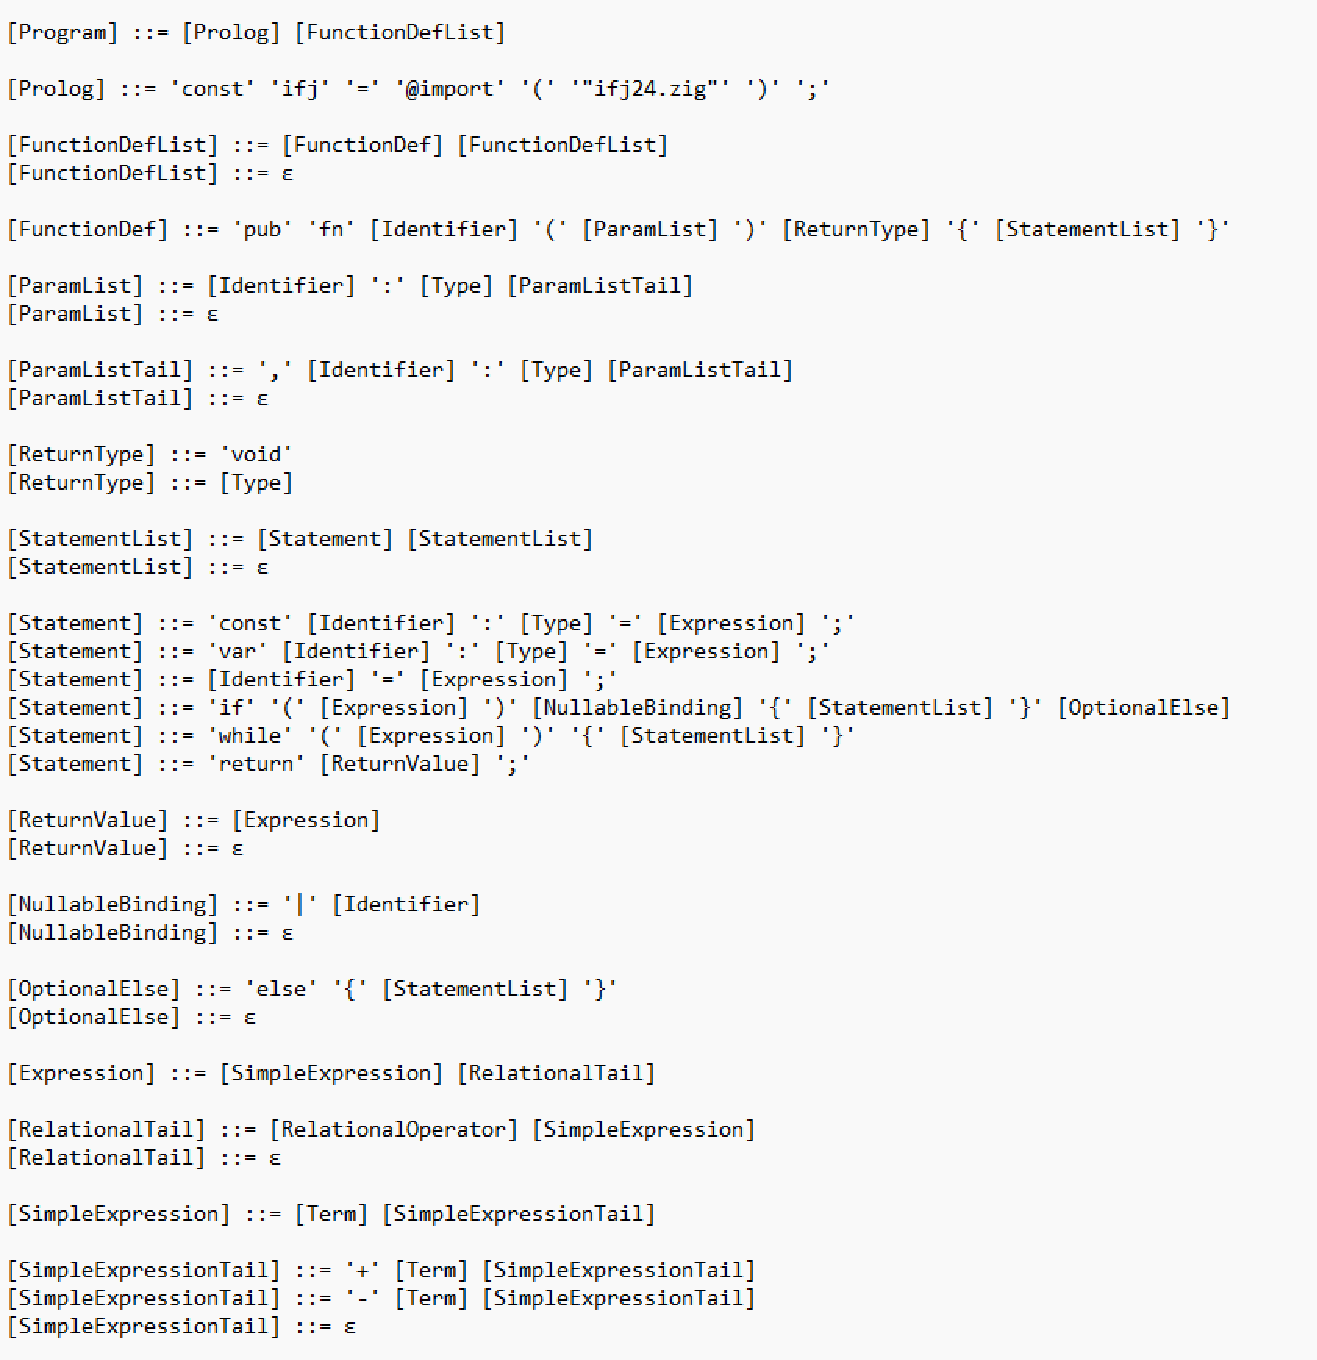
\includegraphics[width=1\linewidth]{Grammar1.pdf}
		\caption{Grammar 1}
		\label{table:png2pdf (1).pdf}
	\end{table}

    
	\begin{table}[!ht]
        \section{Grammar2}
		\centering
		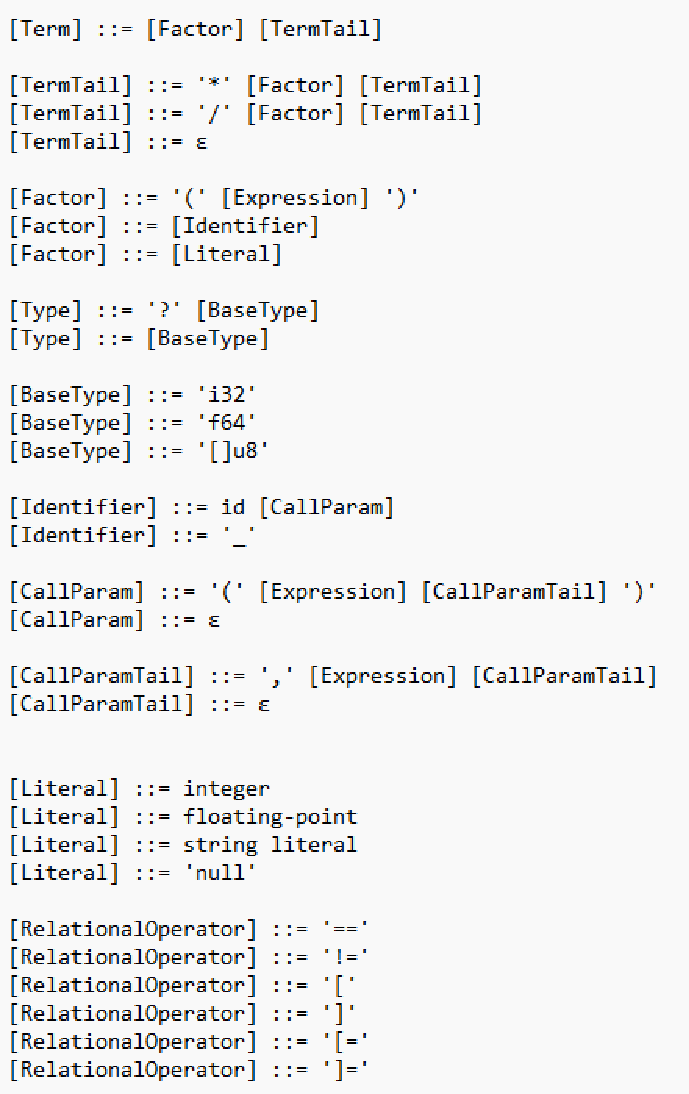
\includegraphics[width=0.7\linewidth]{Grammar2.pdf}
		\caption{Grammar 2}
		\label{table:png2pdf (2).pdf}
	\end{table}


	%\section{LL -- tabulka}
	%\begin{table}[!ht]
	%	\centering
	%	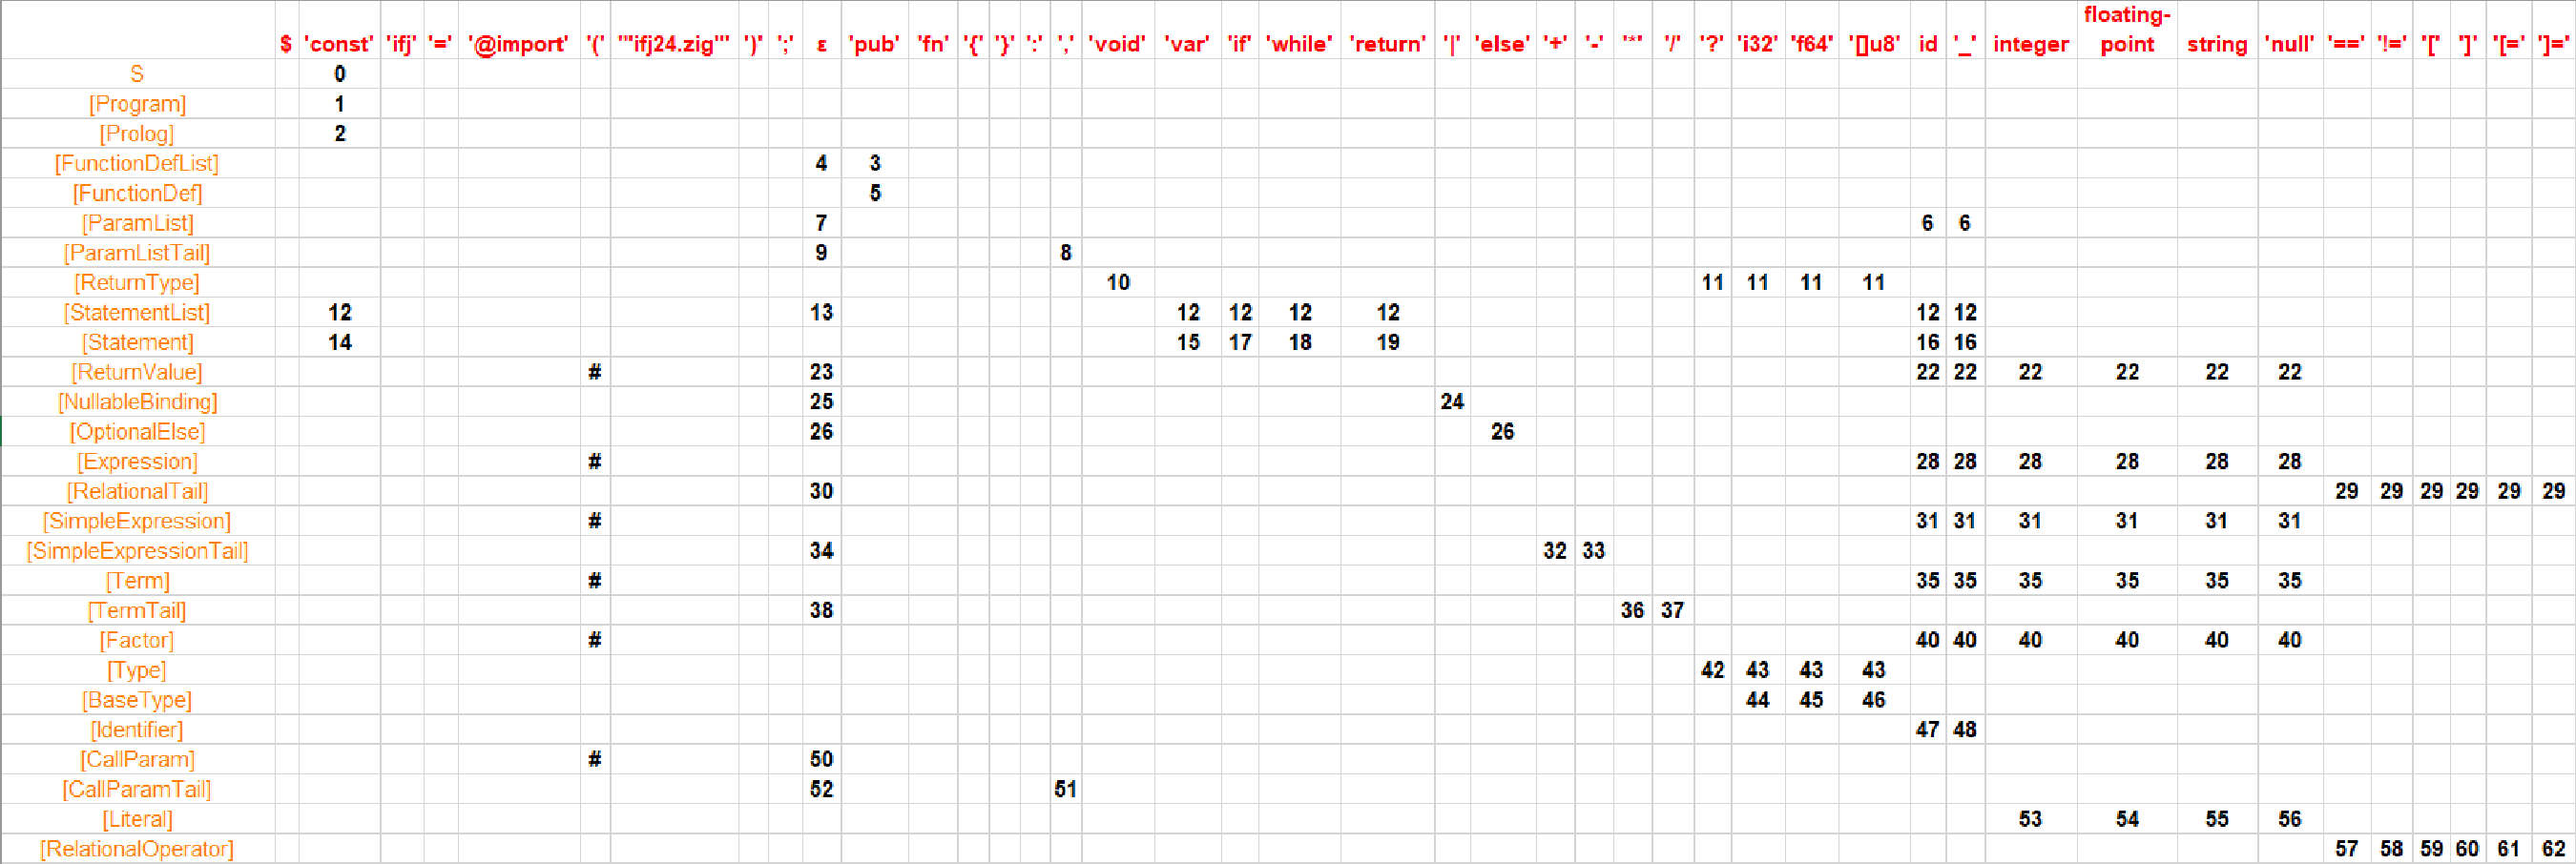
\includegraphics[width=1\linewidth]{inc/LL_table.pdf}
	%	\caption{LL -- tabulka použitá při syntaktické analýze}
	%	\label{table:ll_table}
	%\end{table}


	
	\begin{table}[!ht]
        \section{Precedenční tabulka}
		\centering
		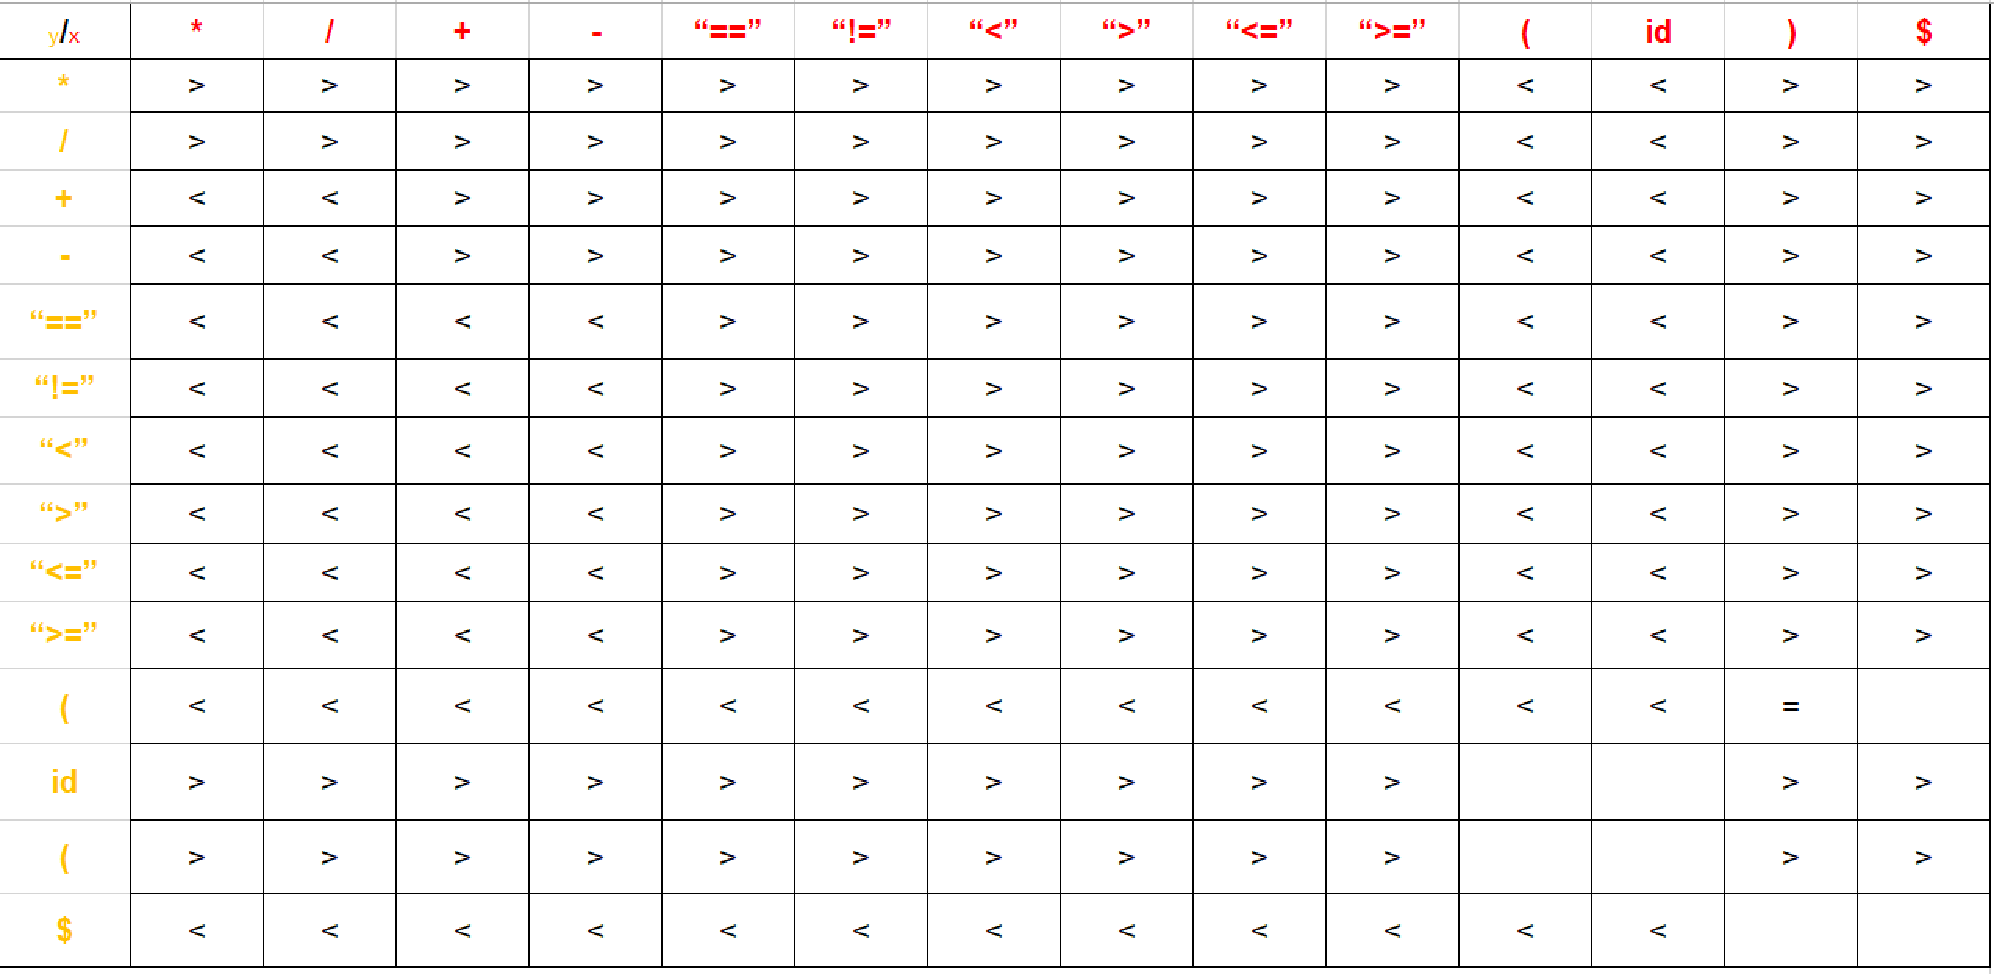
\includegraphics[width=0.7\linewidth]{Precedenční tabulka.pdf}
		\caption{Precedenční tabulka použitá při precedenční syntaktické analýze výrazů}
		\label{table:prec_table}
	\end{table}


\end{document}